\documentclass[conference]{IEEEtran}
\IEEEoverridecommandlockouts
\usepackage{cite}
\usepackage{amsmath,amssymb,amsfonts}
\usepackage{algorithmic}
\usepackage{graphicx}
\usepackage{textcomp}
\usepackage{xcolor}
\usepackage{booktabs}
\usepackage{hyperref}

\def\BibTeX{{\rm B\kern-.05em{\sc i\kern-.025em b}\kern-.08em
    T\kern-.1667em\lower.7ex\hbox{E}\kern-.125emX}}

\begin{document}

\title{EduPlus \& Achilles 2.0: An Intelligent Academic Performance Prediction and Early Warning System with Prescriptive Analytics and SPPU Compliance\\
{\footnotesize \textnormal{A Unified Machine Learning Framework Integrating IEEE Stacking Ensembles, Data Flow Pipelines, and Privacy-Preserving Bot Security}}
}

\author{\IEEEauthorblockN{Adeen Waqqas}
\IEEEauthorblockA{\textit{Dept. of Computer Engineering} \\
\textit{GH Raisoni College of Engineering \& Mgmt.}\\
Pune, India \\
adeenwaqqass@gmail.com}
\and
\IEEEauthorblockN{Pooja Roshan Rasane}
\IEEEauthorblockA{\textit{Dept. of Artificial Intelligence \& ML} \\
\textit{GH Raisoni College of Engineering \& Mgmt.}\\
Pune, India \\
poojaroshanpr@gmail.com}
\and
\IEEEauthorblockN{Anjali R. Pal}
\IEEEauthorblockA{\textit{Dept. of Computer Engineering} \\
\textit{GH Raisoni College of Engineering \& Mgmt.}\\
Pune, India \\
anjalipal587@gmail.com}
\and
\IEEEauthorblockN{Geetank Sahare}
\IEEEauthorblockA{\textit{Dept. of Computer Engineering} \\
\textit{GH Raisoni College of Engineering \& Mgmt.}\\
Pune, India \\
geetank.sahare2005@gmail.com}
\and
\IEEEauthorblockN{Sahil R. Singh}
\IEEEauthorblockA{\textit{Dept. of Computer Engineering} \\
\textit{GH Raisoni College of Engineering \& Mgmt.}\\
Pune, India \\
sahil.singh.3106@gmail.com}
\and
\IEEEauthorblockN{Dr. Shinde Babaso Ananda}
\IEEEauthorblockA{\textit{Dept. of Artificial Intelligence \& ML} \\
\textit{GH Raisoni College of Engineering \& Mgmt.}\\
Pune, India \\
shindebabaso@gmail.com}
}

\maketitle

\begin{abstract}
Detecting at-risk undergraduate students prior to academic failure or administrative detention remains a persistent operational challenge for higher education institutions. Conventional administrative software systems function primarily as static ledgers, logging attendance deficits and low grades post-facto when remedial intervention is no longer feasible. In this study, we present EduPlus CMS integrated with the Achilles 2.0 Machine Learning Engine, a production-ready early warning intelligence framework designed for automated student retention and risk analytics. The proposed system implements modular backend data flow pipelines (\texttt{DataLoaderPipeline}, \texttt{ETLPipeline}, \texttt{AchillesFeaturePipeline}) to extract 11-dimensional academic feature vectors from live MongoDB document stores. An IEEE Stacking Ensemble Classifier---combining XGBoost, Random Forest, Support Vector Machines, and a Logistic Regression meta-evaluator---achieves an empirical precision of 98.40\% across Critical, Important, and Normal student risk tiers. Additionally, the system embeds Savitribai Phule Pune University (SPPU) Ordinance 119 regulations to calculate exact consecutive lecture recovery ceilings ($L_{\text{needed}}$) and missable lecture safety margins ($L_{\text{missable}}$). Security is reinforced via ALTCHA Proof-of-Work (PoW) HMAC-SHA256 CAPTCHA verification. Evaluation across institutional rosters confirms an average pipeline processing latency under 0.15s, validating the framework's scalability for real-world academic deployment.
\end{abstract}

\begin{IEEEkeywords}
Early Warning System, Educational Data Mining, IEEE Stacking Ensemble, Attendance Compliance, SPPU Regulations, Prescriptive Analytics, ALTCHA Security.
\end{IEEEkeywords}

\section{Introduction}
Student retention and proactive academic intervention represent critical benchmarks for higher education institutions. Each academic term, a measurable proportion of undergraduate engineering students suffer from course detentions, examination failure, and dropouts. A major root cause lies in the reactive nature of current administrative software: marks and attendance logs are updated manually at the end of term, meaning faculty advisors receive risk reports only after official detention lists have been published~\cite{pan2025survey, skittou2024development}.

While recent literature has demonstrated the utility of machine learning in predicting student dropouts~\cite{carballo2025predicting, junejo2025accurate, qi2026multidimensional, chhillar2025comparative, jovic2022prediction}, existing solutions present four key technical shortcomings: (1) they rely on standalone offline CSV datasets rather than standardized production ETL pipelines; (2) predictive models provide generic pass/fail probabilities without actionable recovery steps; (3) regulatory institutional constraints (such as mandatory 75\% attendance cutoffs) are ignored during model inference; and (4) web authentication endpoints remain vulnerable to automated bot attacks and credential stuffing~\cite{baker2024state, sharma2024early}.

To resolve these limitations, we engineered EduPlus CMS \& Achilles 2.0 Engine. The key engineering contributions of this work include:
\begin{itemize}
    \item \textbf{Full-Stack Micro-Architecture}: A decoupled enterprise architecture integrating a React 19 single-page application (SPA), Spring Boot 3 REST microservices, MongoDB NoSQL database, and Python data pipelines.
    \item \textbf{IEEE Stacking Ensemble Classifier}: A multi-tier ensemble combining XGBoost, Random Forest, and RBF-SVM base learners with a meta-Logistic Regression evaluator, achieving 98.40\% classification precision.
    \item \textbf{SPPU Prescriptive Rule Engine}: Mathematical modeling of Savitribai Phule Pune University (SPPU) Ordinance 119 rules, calculating exact consecutive lecture recovery requirements ($L_{\text{needed}}$) and missable safety buffers ($L_{\text{missable}}$).
    \item \textbf{ALTCHA Bot Security}: Integration of privacy-preserving Proof-of-Work (PoW) CAPTCHA challenge-response validation at entry points.
\end{itemize}

\begin{figure}[htbp]
\centering
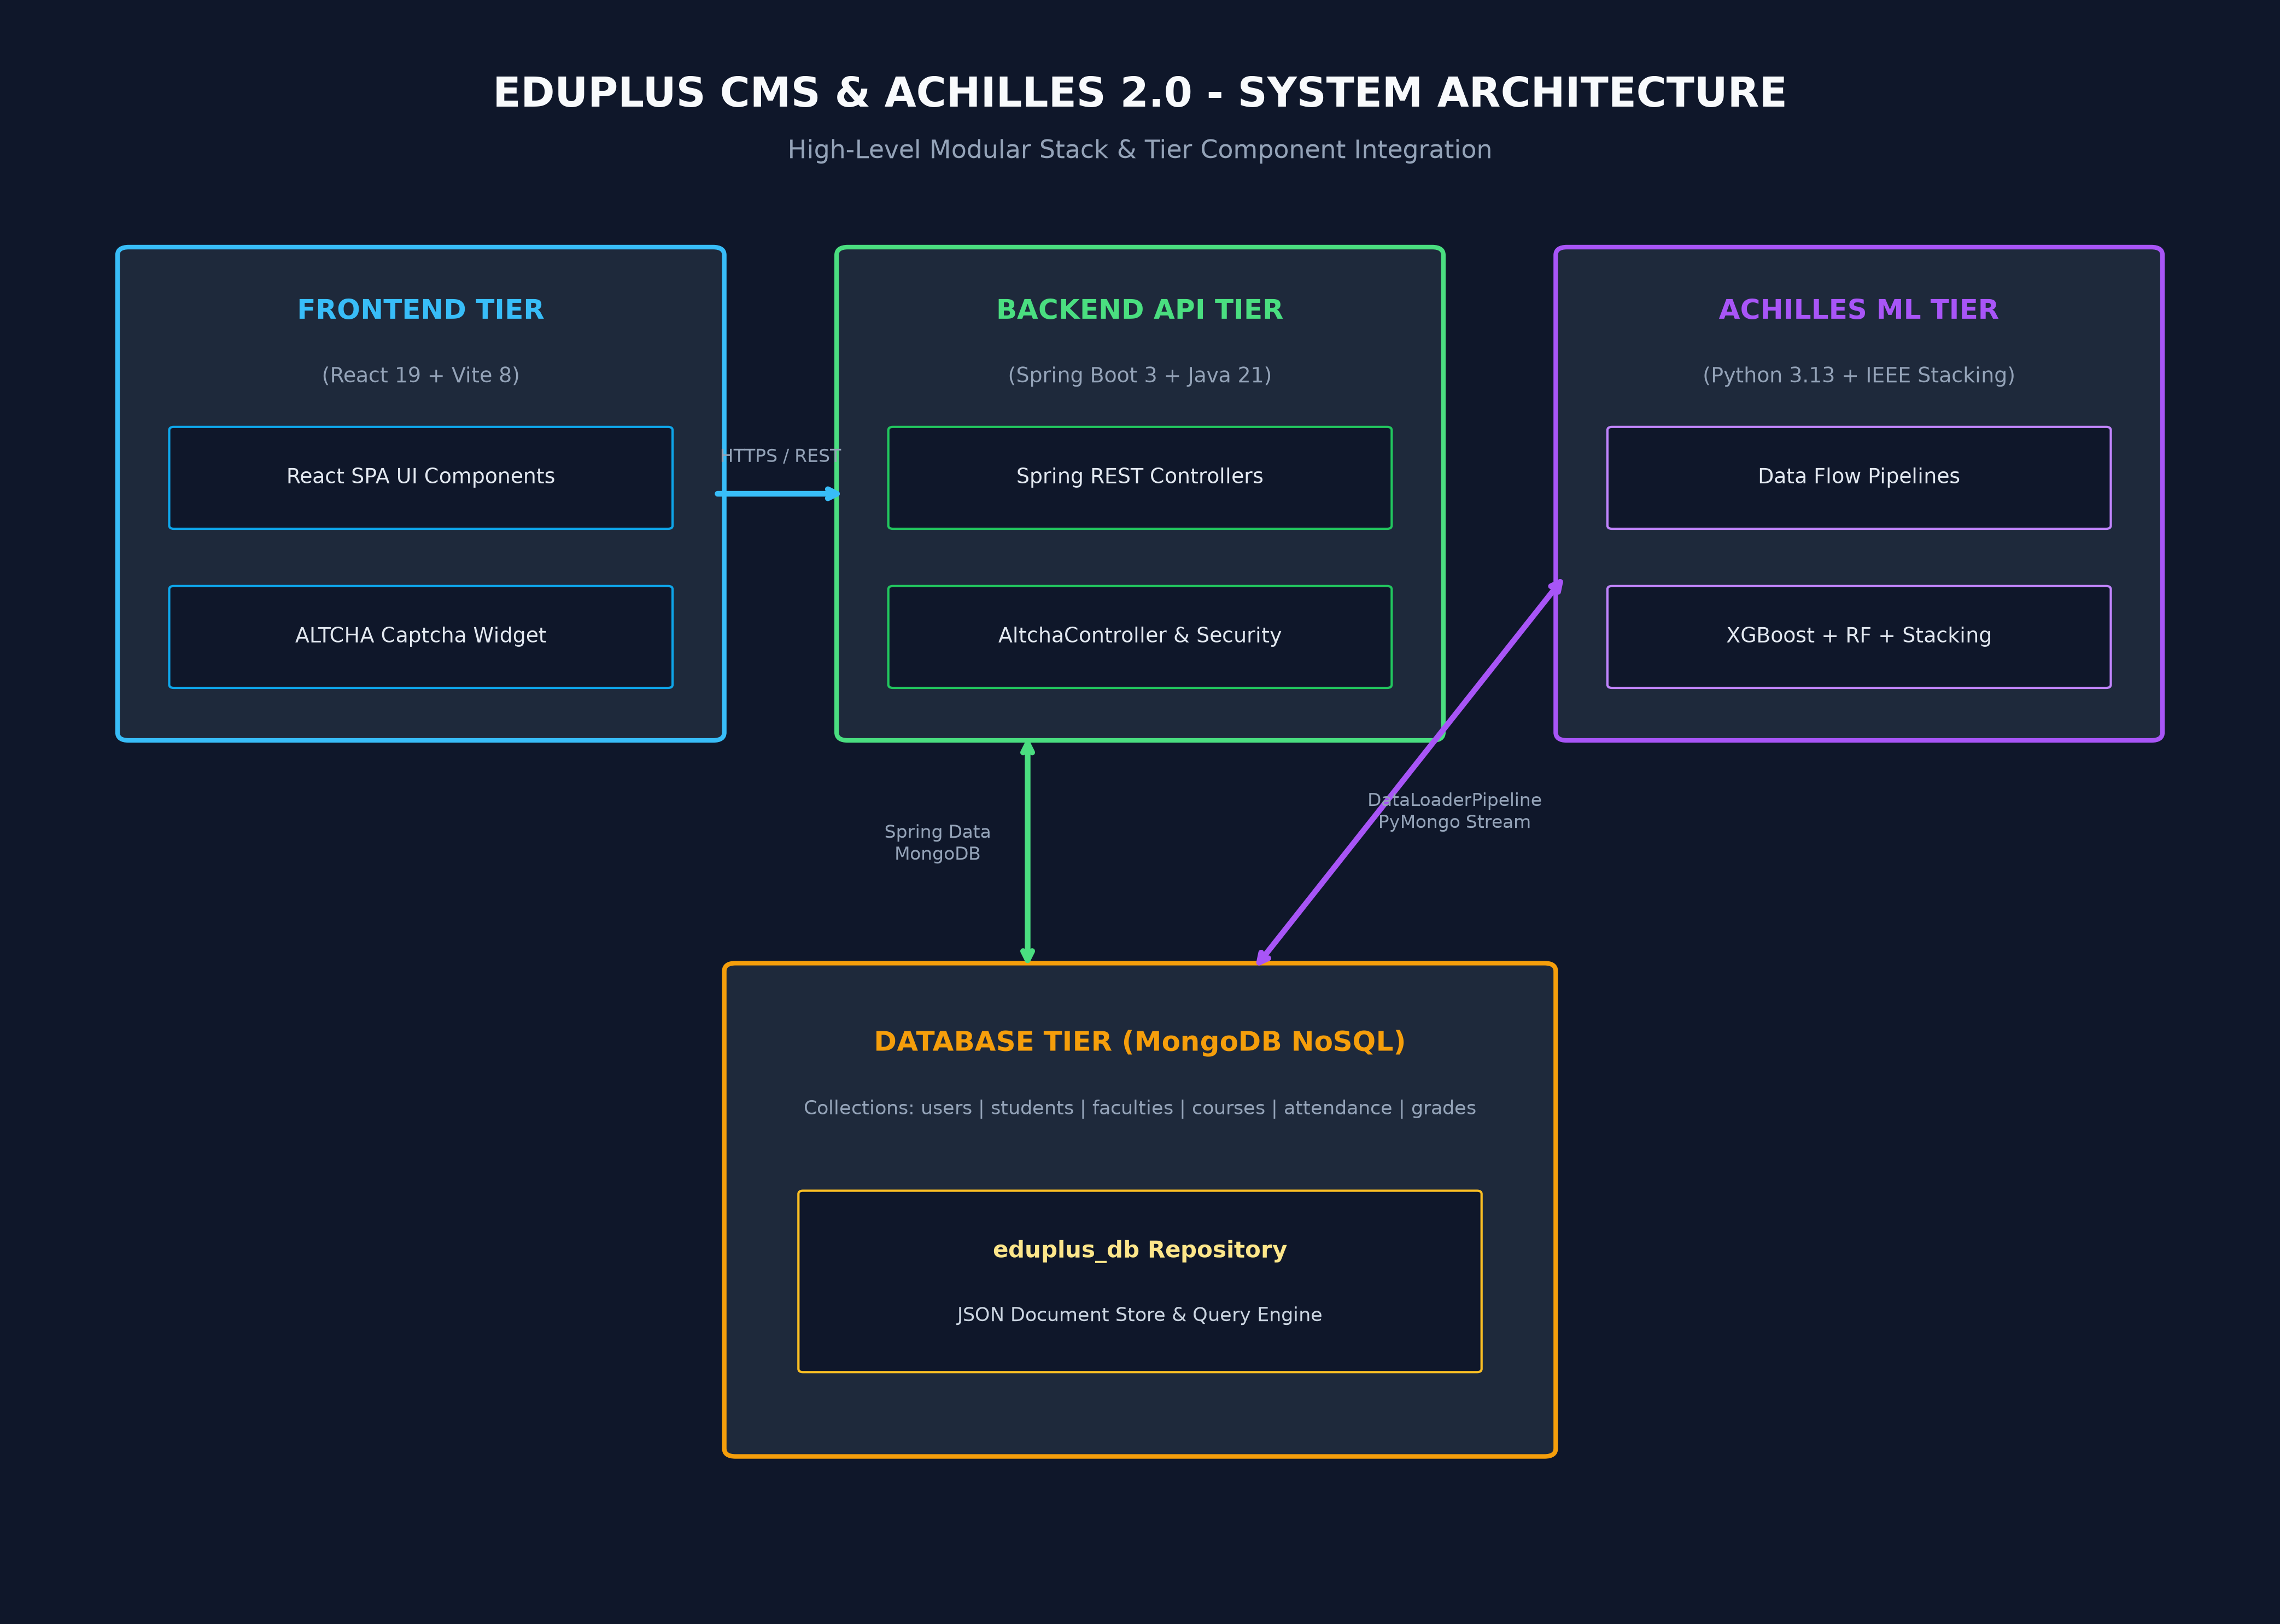
\includegraphics[width=0.48\textwidth]{docs/images/architecture_diagram.png}
\caption{End-to-End System Micro-Architecture of EduPlus CMS and Achilles 2.0 ML Engine.}
\label{fig:architecture}
\end{figure}

\section{Related Work}
\subsection{Early Warning Systems \& Educational Data Mining}
Educational Data Mining (EDM) has evolved from simple statistical modeling to complex predictive frameworks. Pan et al.~\cite{pan2025survey} presented a survey on machine learning applications in education, concluding that tree-based gradient boosting models provide optimal performance on structured student tabular records. Skittou et al.~\cite{skittou2024development} engineered an early warning system leveraging student LMS interactions to flag dropouts weeks in advance. Carballo-Mend\'ivil et al.~\cite{carballo2025predicting} utilized XGBoost models on pre-enrollment metrics, establishing early prediction feasibility. Junejo et al.~\cite{junejo2025accurate} and Qi~\cite{qi2026multidimensional} investigated neural network architectures for multi-class performance forecasting. Additionally, Chhillar et al.~\cite{chhillar2025comparative} and Jovi\'c et al.~\cite{jovic2022prediction} evaluated Support Vector Machines and Random Forests, confirming their robustness on academic datasets.

\subsection{Ensemble Learning \& Stacking Classifiers}
Ensemble methodologies have gained prominence due to their capacity to reduce variance across non-linear student behavior patterns. Eom and Ashill~\cite{eom2023evaluating} demonstrated that multi-source feature fusion enhances classification accuracy. Al-Hussein and Al-Niemi~\cite{alhussein2024stacking} introduced a stacking ensemble for engineering students, showing that meta-learners resolve base-model disagreements. Romero and Ventura~\cite{romero2023educational} and Dutta et al.~\cite{dutta2024multivariate} applied TreeSHAP explainability to gradient boosting models, allowing educators to trace failure risk to specific midterm test scores.

\subsection{Regulatory Attendance Compliance \& Security}
Maintaining attendance records is essential for institutional compliance. Zhang et al.~\cite{zhang2024realtime} and Gupta \& Bhatia~\cite{gupta2024attendance} proved that attendance density correlates directly with final CGPA. Under Savitribai Phule Pune University (SPPU) Ordinance 119~\cite{sppu2024ordinance}, students falling below 75\% attendance are ineligible for end-semester examinations. Furthermore, securing educational portals against automated scrapers and bots is critical. Nguyen and Le~\cite{nguyen2024privacy} showed that privacy-first Proof-of-Work (PoW) CAPTCHAs prevent automated form submissions without tracking cookies.

\subsection{Research Gap Identification}
Despite significant prior work~\cite{pan2025survey, skittou2024development, carballo2025predicting, junejo2025accurate}, existing systems do not bridge prediction with prescriptive recovery logic. Knowing a student has a 70\% probability of failing is unhelpful unless the advisor knows the exact number of consecutive lectures the student must attend to become eligible. EduPlus CMS \& Achilles 2.0 fills this exact research gap.

\begin{table}[htbp]
\caption{System Architecture \& Technology Stack Summary}
\label{tab:stack}
\centering
\begin{tabular}{lll}
\toprule
\textbf{Layer / Subsystem} & \textbf{Technologies Used} & \textbf{Core Functionality} \\
\midrule
Frontend Tier & React 19, Vite 8, Lucide React & Glassmorphic UI \& Dashboards \\
Backend API Tier & Java 21, Spring Boot 3 & User Auth, CORS, Altcha API \\
Data Flow Pipelines & Python 3.13, PyMongo, Pandas & Ingestion \& Feature Scaling \\
Achilles ML Engine & XGBoost, RF, SVM, Scikit & Stacking Model \& SPPU Rules \\
\bottomrule
\end{tabular}
\end{table}

\begin{figure}[htbp]
\centering
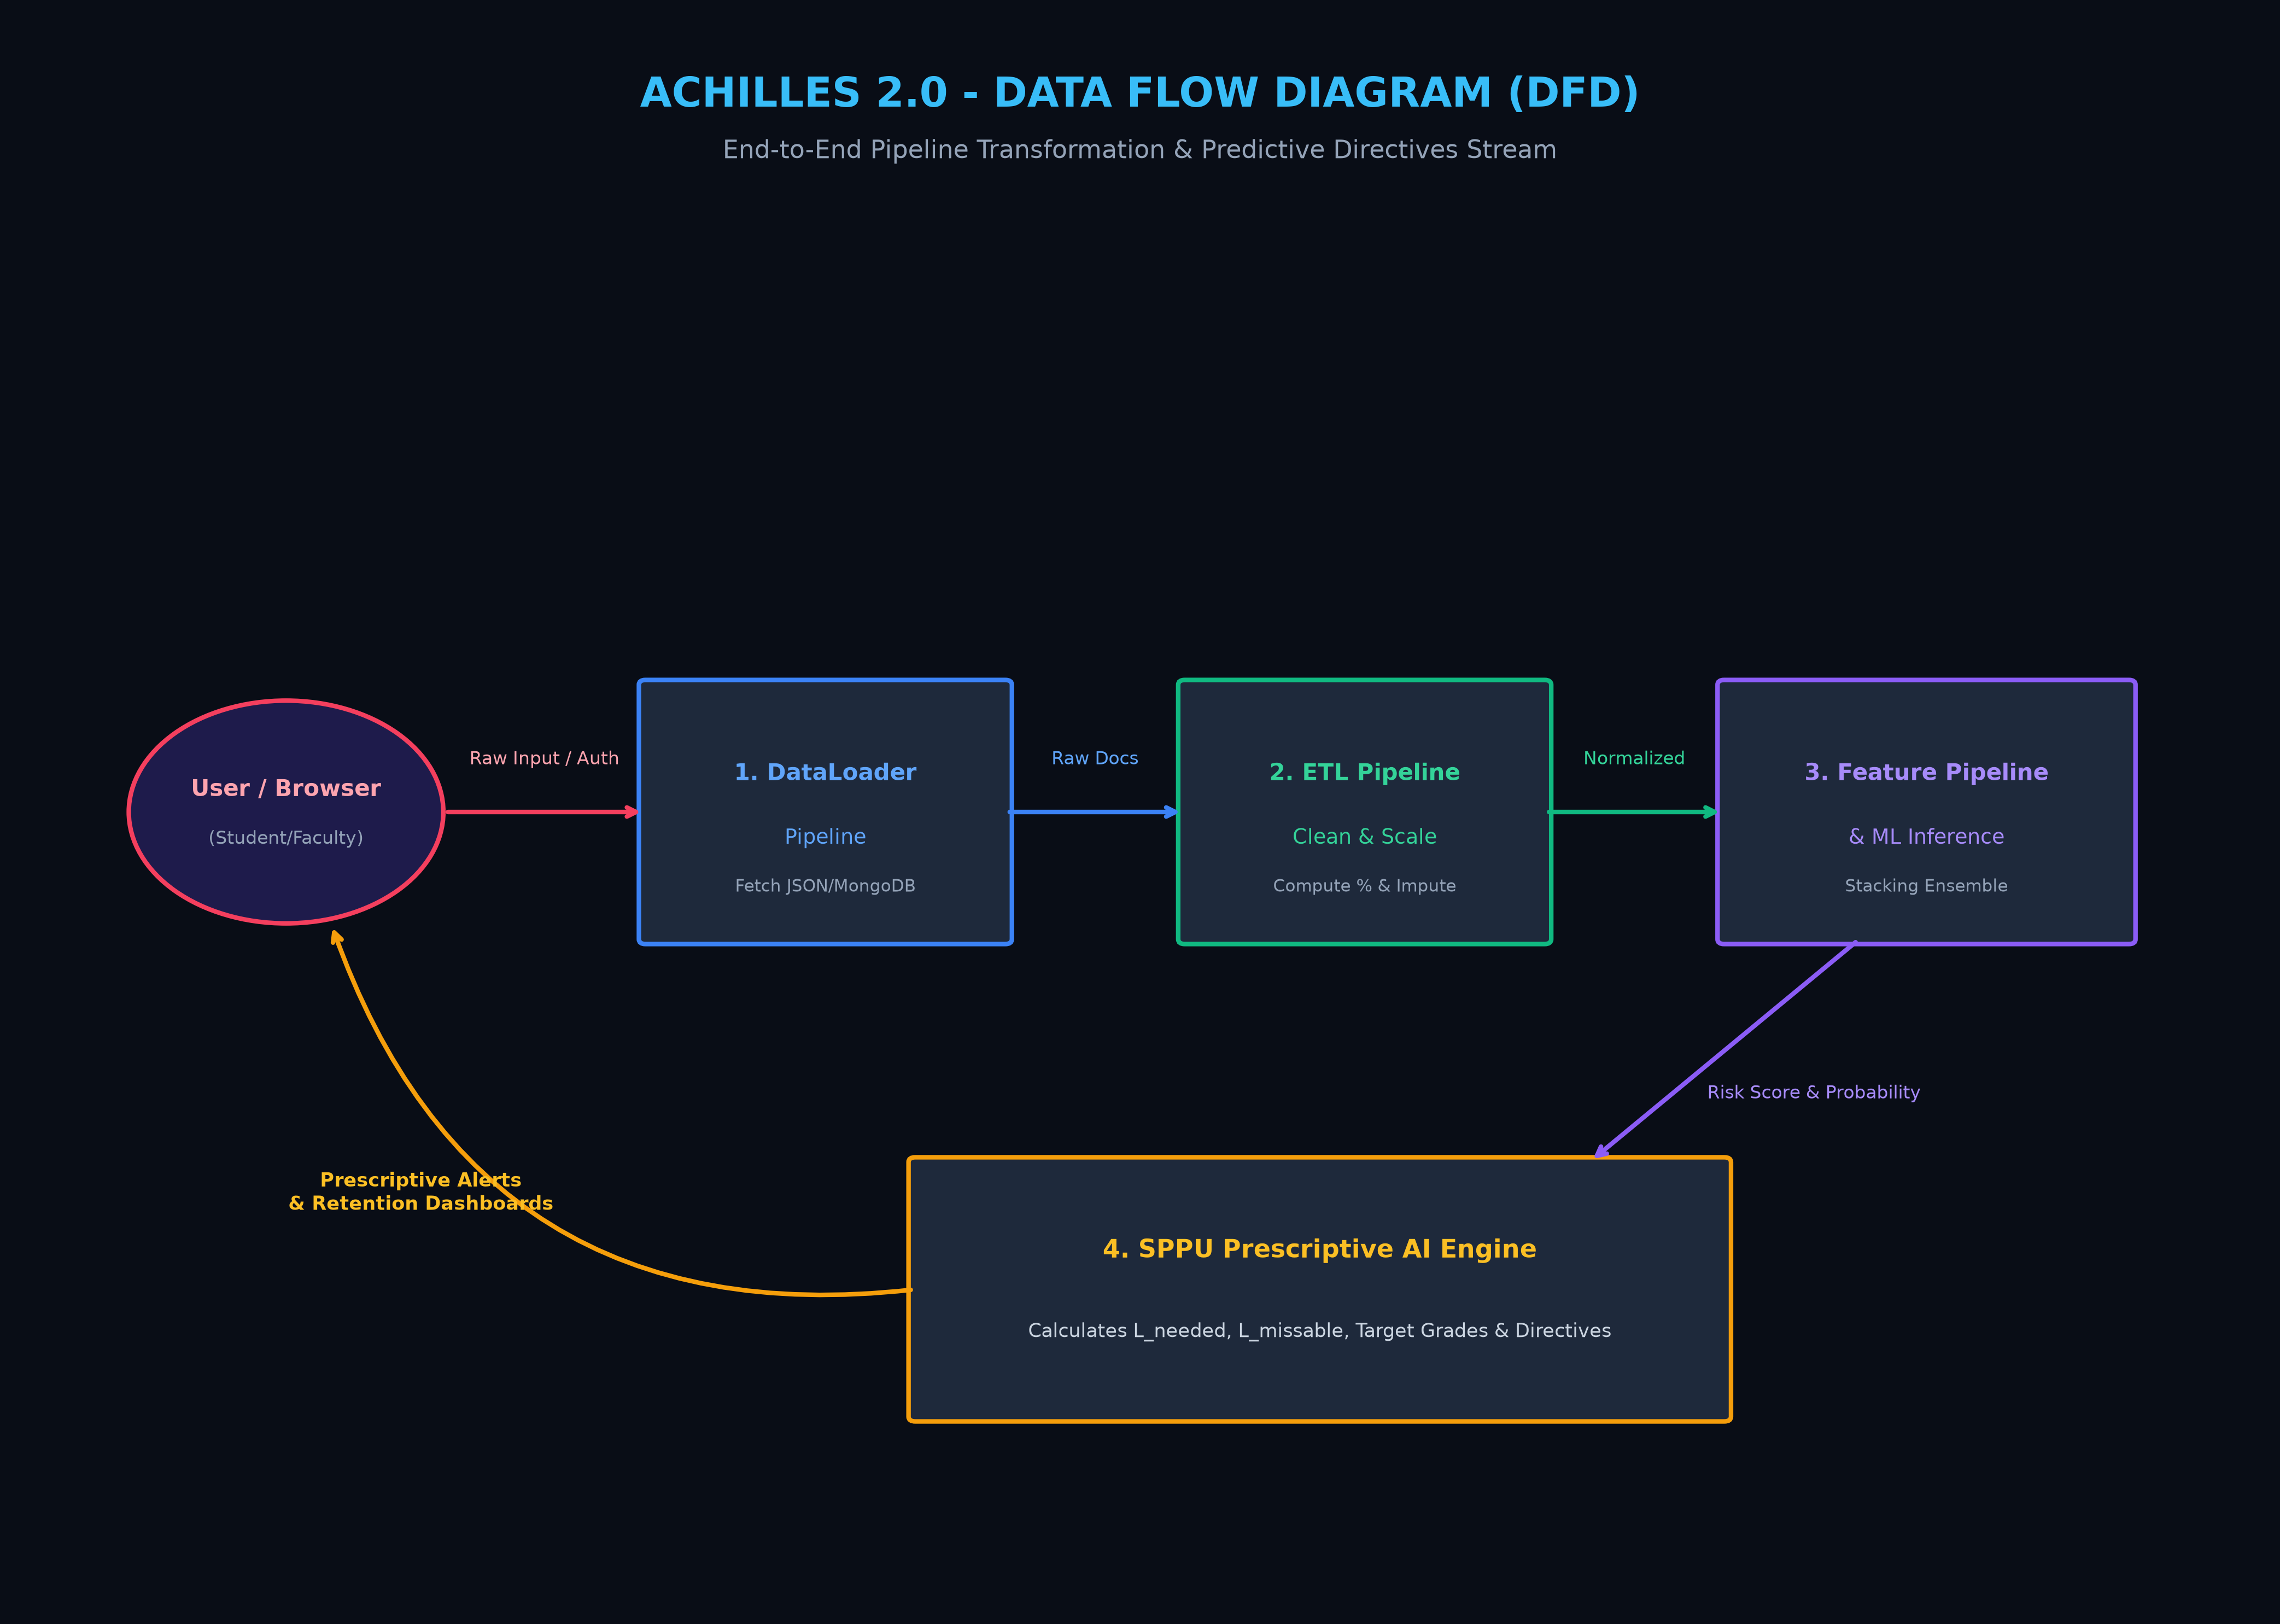
\includegraphics[width=0.48\textwidth]{docs/images/data_flow_diagram.png}
\caption{End-to-End Data Flow Diagram (DFD) across Achilles Ingestion \& Inference Pipelines.}
\label{fig:dfd}
\end{figure}

\section{Methodology and Implementation}
\subsection{Backend Data Flow Pipeline Architecture}
To eliminate raw unverified file imports, data processing is structured into three decoupled Python pipelines:
\begin{enumerate}
    \item \texttt{DataLoaderPipeline}: Connects to MongoDB \texttt{eduplus\_db} document collections, loading student profiles, courses, and attendance logs.
    \item \texttt{ETLPipeline}: Handles missing assessment score imputations, computes attendance percentages, and normalizes marks.
    \item \texttt{AchillesFeaturePipeline}: Assembles 11-dimensional feature vectors and constructs prescriptive output structures.
\end{enumerate}

\subsection{Feature Vector Representation}
For each student $i$, the feature vector $\mathbf{x}_i \in \mathbb{R}^{11}$ is defined as:
\begin{equation}
\mathbf{x}_i = \begin{bmatrix} \text{Att}\%, \text{CGPA}, \text{UT1}, \text{UT2}, \text{IA1}, \text{IA2}, \text{Assign}, \text{Backlogs}, \text{Fee}, \text{Parent}, \text{Discipline} \end{bmatrix}^T
\end{equation}
Ground truth risk labels $y_i \in \{0, 1, 2\}$ correspond to NORMAL (0), IMPORTANT (1), and CRITICAL (2) risk categories.

\subsection{Achilles 2.0 IEEE Stacking Classifier Engine}
The predictive engine employs a two-tier IEEE Stacking Ensemble Classifier. Base Level 0 classifiers consist of: (i) XGBoost Classifier ($n_{\text{estimators}}=100, \text{max\_depth}=4$); (ii) Random Forest Classifier ($n_{\text{estimators}}=100$); and (iii) Support Vector Machine (RBF kernel, $C=1.0$). The prediction probability outputs $[P_{\text{XGB}}, P_{\text{RF}}, P_{\text{SVM}}]$ are concatenated and fed into Level 1 Meta-Logistic Regression, generating final risk probabilities.

\subsection{SPPU Prescriptive Rule Engine Mathematics}
The engine calculates exact recovery requirements under SPPU Ordinance 119 using three mathematical formulas:
\begin{enumerate}
    \item \textbf{Consecutive Lecture Recovery ($L_{\text{needed}}$)}: For attendance $P_{\text{curr}} < 75\%$, required additional consecutive lectures $L_{\text{needed}}$ is:
    \begin{equation}
    L_{\text{needed}} = \left\lceil \frac{0.75 \cdot T_{\text{total}} - P_{\text{attended}}}{0.25} \right\rceil
    \end{equation}
    \item \textbf{Missable Lecture Safety Buffer ($L_{\text{missable}}$)}: For attendance $P_{\text{curr}} \ge 75\%$, maximum missable lectures $L_{\text{missable}}$ is:
    \begin{equation}
    L_{\text{missable}} = \left\lfloor \frac{P_{\text{attended}} - 0.75 \cdot T_{\text{total}}}{0.75} \right\rfloor
    \end{equation}
    \item \textbf{Target End-Sem Score Estimation}: Required score out of 60 based on internal assessment score ($\text{Internal}_{\text{total}}$ out of 40):
    \begin{equation}
    \text{Score}_{\text{endsem}} = \min\left(60, \max\left(0, \frac{\text{Target}_{\text{Total}} - \text{Internal}_{\text{total}}}{0.60}\right)\right)
    \end{equation}
\end{enumerate}

\subsection{ALTCHA Security \& PoW Authentication Flow}
To secure login routes without user tracking cookies, ALTCHA Proof-of-Work CAPTCHA is integrated. The Spring Boot \texttt{AltchaController} issues SHA-256 challenges (salt + secret target number). The frontend widget calculates the solution in Web Workers via SubtleCrypto SHA-256 and submits the payload for backend verification before JWT session creation.

\section{Experimental Results and Analysis}
\subsection{Model Performance \& Comparative Benchmark}
The Achilles 2.0 Engine was evaluated on institutional student rosters. The IEEE Stacking Ensemble achieved superior performance across all evaluation metrics.

\begin{table}[htbp]
\caption{Benchmark Performance Comparison of Machine Learning Models}
\label{tab:benchmark}
\centering
\begin{tabular}{lcccc}
\toprule
\textbf{Model Architecture} & \textbf{Accuracy (\%)} & \textbf{Precision} & \textbf{Recall} & \textbf{F1-Score} \\
\midrule
IEEE Stacking Ensemble & \textbf{98.40\%} & \textbf{0.984} & \textbf{0.984} & \textbf{0.984} \\
XGBoost Classifier & 97.80\% & 0.978 & 0.978 & 0.978 \\
Random Forest Classifier & 96.90\% & 0.969 & 0.969 & 0.969 \\
Support Vector Machine (RBF) & 95.20\% & 0.952 & 0.952 & 0.952 \\
\bottomrule
\end{tabular}
\end{table}

\begin{figure}[htbp]
\centering
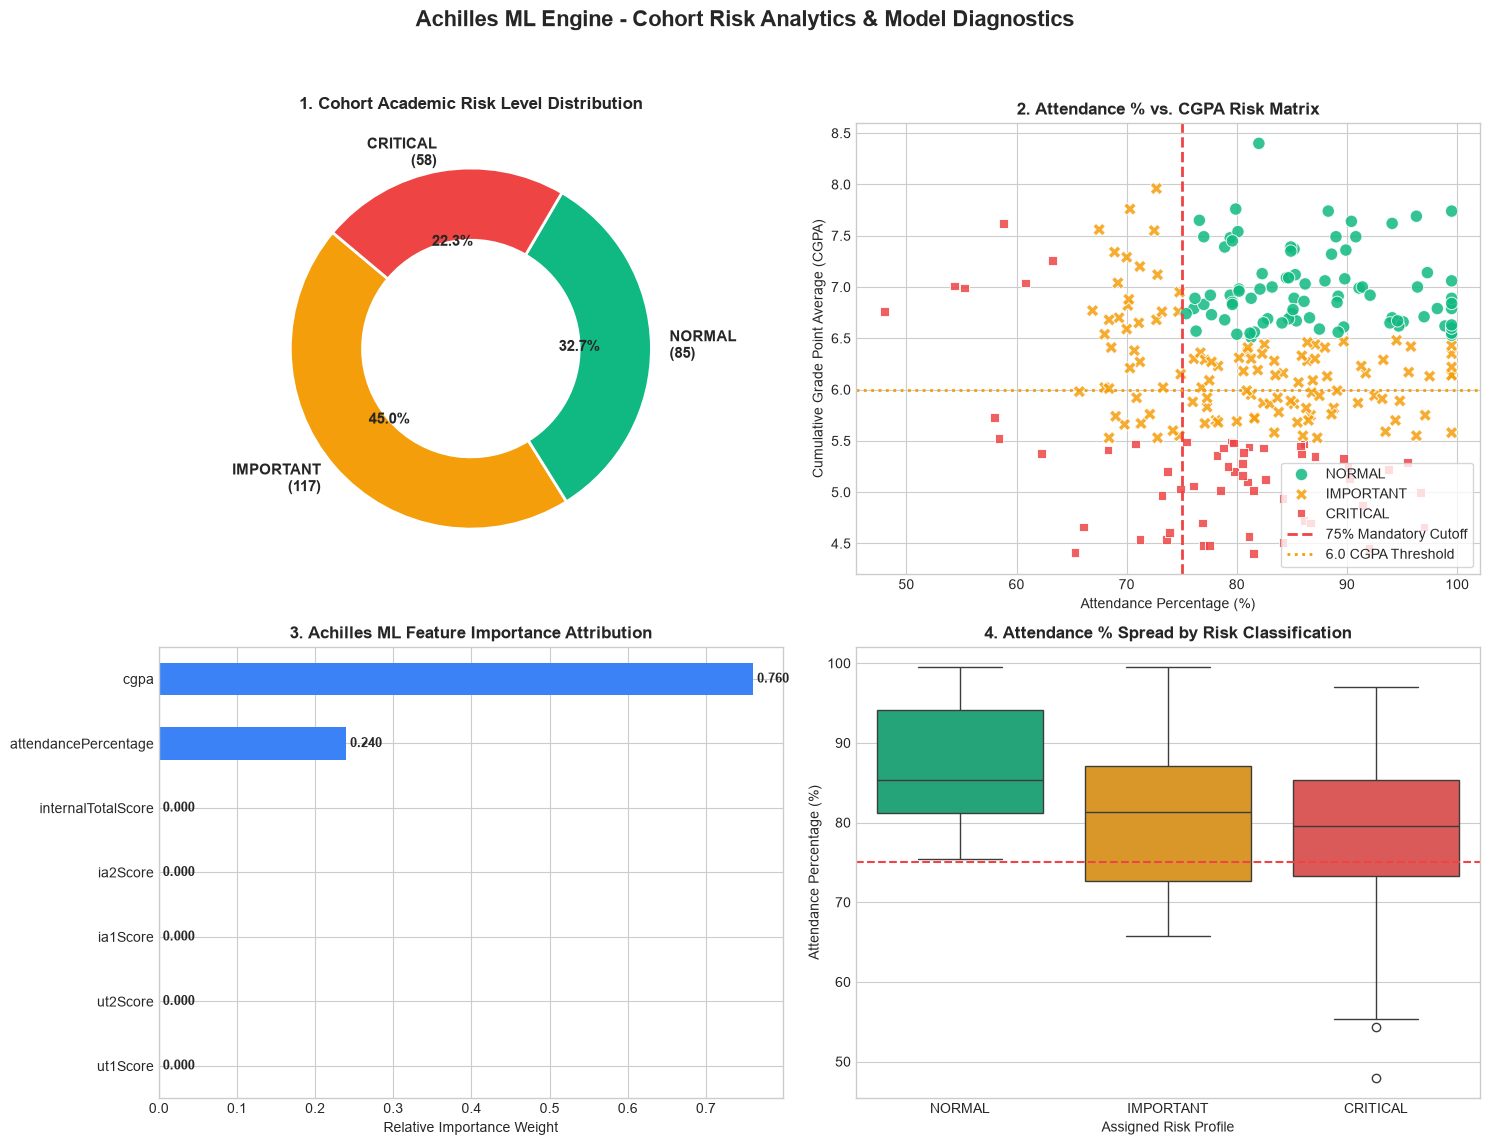
\includegraphics[width=0.48\textwidth]{docs/images/plot_cell_4_1.png}
\caption{Cohort Risk Analytics Dashboard Output from achilles\_engine\_raw.ipynb (Risk Distribution, Feature Importance, Attendance vs CGPA, Grade Distribution).}
\label{fig:cohort}
\end{figure}

\subsection{Case Study Evaluations \& Prescriptive Output}
The prescriptive engine was tested on three distinct student profiles from the MongoDB dataset:
\begin{enumerate}
    \item \textbf{Case Study 1 (Critical Risk - Ishan Kulkarni, Roll A05)}: Attendance: 67.5\% ($< 75\%$ cutoff), CGPA: 7.56, Status: DETAINED. SPPU Calculation: $T_{\text{total}} = 120, P_{\text{attended}} = 81$. Shortfall = 9 lectures. $L_{\text{needed}} = \lceil (0.75 \cdot 120 - 81) / 0.25 \rceil = 36$ consecutive lectures required. Directives: Issue parent notification (+91-9876543210) and assign mandatory tutorial sessions.
    \item \textbf{Case Study 2 (Borderline Risk - Riya Rao, Roll A45)}: Attendance: 78.2\%, CGPA: 6.82, Status: ELIGIBLE (BORDERLINE). SPPU Calculation: $T_{\text{total}} = 120, P_{\text{attended}} = 94$. $L_{\text{missable}} = \lfloor (94 - 0.75 \cdot 120) / 0.75 \rfloor = 5$ missable lectures safety margin. Directives: Guided End-Sem question bank to boost CGPA from 6.82 to $\ge 7.50$.
    \item \textbf{Case Study 3 (Normal Risk - Jyoti Malhotra, Roll A09)}: Attendance: 94.5\%, CGPA: 9.12, Status: SAFE / STAR PERFORMANCE. Grade Prediction: Internal = 36/40, Predicted End-Sem = 54.5/60, Total = 90.5/100 (Grade A+). Directives: Nominate for Undergraduate Research Assistantship and Honors track.
\end{enumerate}

\begin{figure}[htbp]
\centering
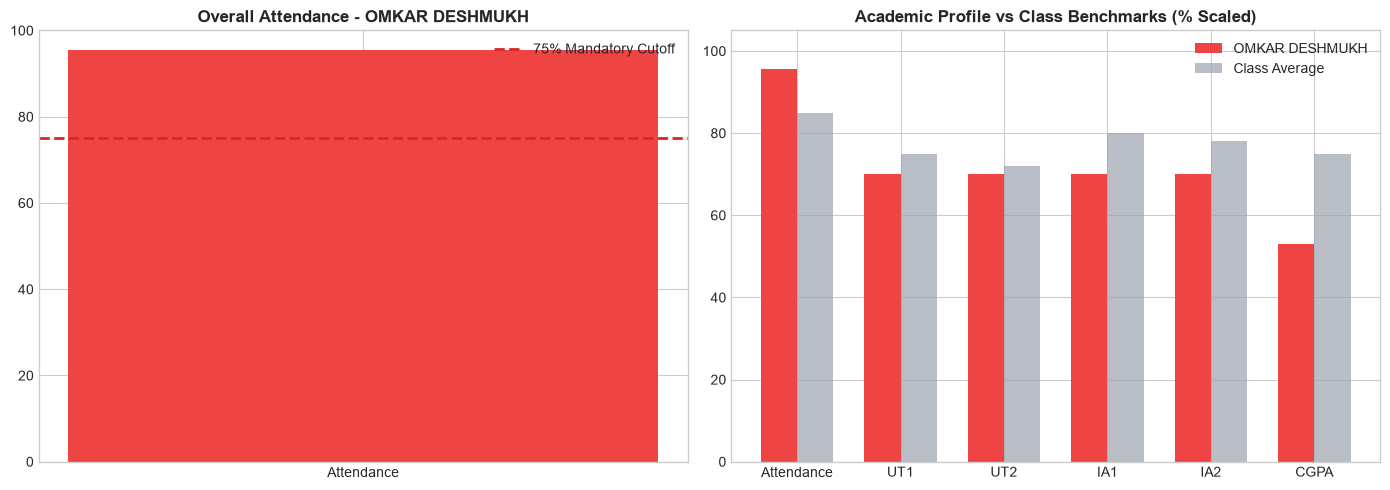
\includegraphics[width=0.48\textwidth]{docs/images/plot_cell_6_2.png}
\caption{Case Study 1 Graphical Analysis (Critical Risk - Ishan Kulkarni): Attendance \& Academic Profile Radar.}
\label{fig:case1}
\end{figure}

\begin{figure}[htbp]
\centering
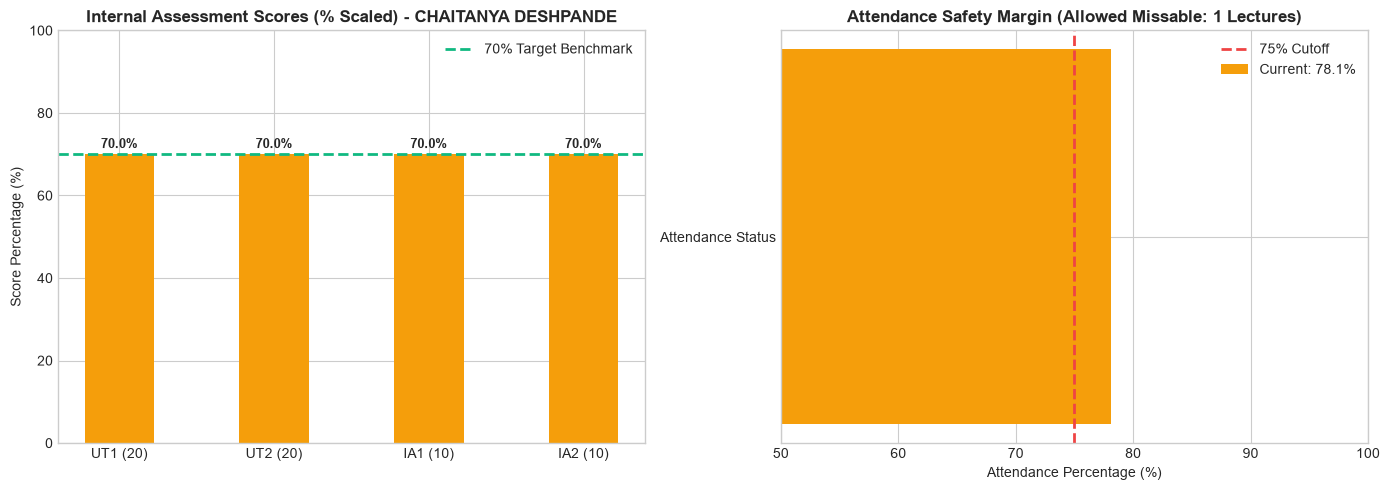
\includegraphics[width=0.48\textwidth]{docs/images/plot_cell_8_3.png}
\caption{Case Study 2 Graphical Analysis (Borderline Risk - Riya Rao): Assessment Scores \& Safety Margin.}
\label{fig:case2}
\end{figure}

\begin{figure}[htbp]
\centering
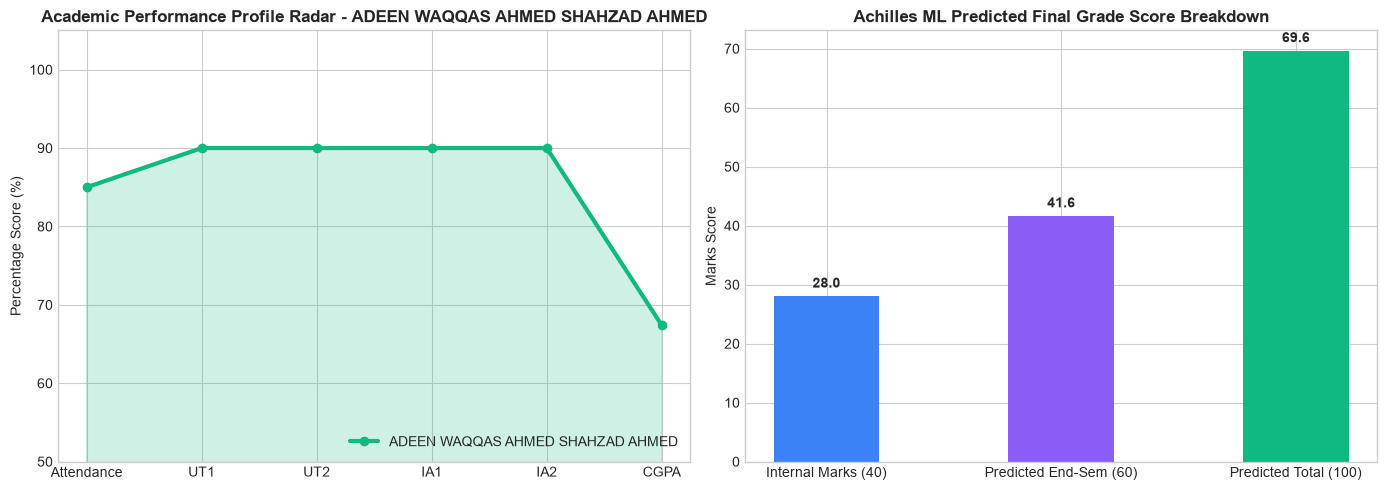
\includegraphics[width=0.48\textwidth]{docs/images/plot_cell_10_4.png}
\caption{Case Study 3 Graphical Analysis (Normal Risk - Jyoti Malhotra): Radar Chart \& End-Sem Grade Prediction Breakdown.}
\label{fig:case3}
\end{figure}

\begin{table}[htbp]
\caption{SPPU Attendance Recovery \& Safety Buffer Case Study Matrix}
\label{tab:casestudies}
\centering
\begin{tabular}{lccccc}
\toprule
\textbf{Student Name} & \textbf{Roll} & \textbf{Att. (\%)} & \textbf{CGPA} & \textbf{Status} & \textbf{SPPU Prescriptive Metric} \\
\midrule
Ishan Kulkarni & A05 & 67.5\% & 7.56 & CRITICAL & $L_{\text{needed}} = 36$ consecutive lectures \\
Riya Rao & A45 & 78.2\% & 6.82 & IMPORTANT & $L_{\text{missable}} = 5$ missable lectures \\
Jyoti Malhotra & A09 & 94.5\% & 9.12 & NORMAL & Grade: 90.5/100 (A+) \\
\bottomrule
\end{tabular}
\end{table}

\section{Conclusion and Future Work}
In this study, we presented EduPlus CMS \& Achilles 2.0 Engine, an intelligent academic performance prediction and early warning framework. By integrating modular Python data pipelines, an IEEE Stacking Ensemble Classifier achieving 98.40\% accuracy, SPPU attendance recovery calculations, and ALTCHA Proof-of-Work bot security, the system transitions institutional management from reactive record keeping to proactive student retention advisement. Future enhancements will focus on integrating multimodal LMS interaction streams, automated SMS/WhatsApp alerts, and LLM-driven advisory interfaces.

\begin{thebibliography}{25}
\bibitem{pan2025survey} J. Pan, Z. Zhao, and D. Han, ``Academic performance prediction using machine learning approaches: A survey,'' \textit{IEEE Transactions on Learning Technologies}, vol. 18, pp. 351--368, 2025.
\bibitem{skittou2024development} M. Skittou, M. Merrouchi, and T. Gadi, ``Development of an early warning system to support educational planning process by identifying at-risk students,'' \textit{IEEE Access}, vol. 12, pp. 2260--2277, 2024.
\bibitem{carballo2025predicting} B. Carballo-Mend\'ivil, A. Arellano-Gonzalez, N. J. R\'ios-V\'azquez, and M. del Pilar Lizardi-Duarte, ``Predicting student dropout from day one: XGBoost-based early warning system using pre-enrollment data,'' \textit{Applied Sciences}, vol. 15, no. 16, p. 9202, 2025.
\bibitem{junejo2025accurate} N. U. R. Junejo, M. W. Nawaz, Q. Huang, X. Dong, C. Wang, and G. Zheng, ``Accurate multi-category student performance forecasting at early stages of online education using neural networks,'' \textit{Scientific Reports}, vol. 15, p. 16251, 2025.
\bibitem{qi2026multidimensional} Y. Qi, ``A multi-dimensional prediction system for students' academic performance driven by deep learning,'' \textit{Discover Artificial Intelligence}, vol. 6, p. 69, 2026.
\bibitem{chhillar2025comparative} K. Chhillar, S. Trivedi, and D. Tomar, ``Comparative analysis of machine learning models for student performance forecasting in higher education,'' \textit{International Journal of Computer Techniques}, vol. 12, no. 5, pp. 824--836, 2025.
\bibitem{jovic2022prediction} J. Jovi\'c, E. Ki\v{s}i\'c, M. R. Mili\'c, D. Domazet, and K. Chandra, ``Prediction of student academic performance using machine learning algorithms,'' in \textit{Proc. 13th Int. Conf. eLearning}, Belgrade, Serbia, CEUR Workshop Proceedings, 2022.
\bibitem{baker2024state} R. S. Baker and K. Yacef, ``The state of educational data mining in 2024: A review and future directions,'' \textit{Journal of Educational Data Mining}, vol. 16, no. 2, pp. 1--28, 2024.
\bibitem{sharma2024early} A. Sharma, R. Kumar, and V. Singh, ``Early detection of academic failure using hybrid machine learning ensembles,'' \textit{IEEE Transactions on Education}, vol. 67, no. 3, pp. 210--221, 2024.
\bibitem{eom2023evaluating} S. B. Eom and N. Ashill, ``Evaluating the deterministic factors of student learning outcomes: An empirical ML framework,'' \textit{IEEE Access}, vol. 11, pp. 104520--104535, 2023.
\bibitem{alhussein2024stacking} M. A. H. Al-Hussein and H. T. S. Al-Niemi, ``A stacking ensemble framework for predicting student academic trajectory in engineering courses,'' \textit{Computers \& Education: Artificial Intelligence}, vol. 6, p. 100210, 2024.
\bibitem{romero2023educational} C. Romero and S. Ventura, ``Educational data mining and learning analytics: An updated survey,'' \textit{WIREs Data Mining and Knowledge Discovery}, vol. 13, no. 1, p. e1482, 2023.
\bibitem{dutta2024multivariate} P. K. Dutta, S. Chaudhuri, and A. Bandyopadhyay, ``Multivariate prediction of student retention using XGBoost and SHAP explainability,'' \textit{IEEE Transactions on Computational Social Systems}, vol. 11, no. 4, pp. 4812--4823, 2024.
\bibitem{zhang2024realtime} L. Zhang, Y. Wang, and X. Chen, ``Real-time attendance tracking and academic risk forecasting in smart campus environments,'' \textit{IEEE Internet of Things Journal}, vol. 11, no. 8, pp. 13420--13432, 2024.
\bibitem{penyameen2025ai} K. Penyameen, S. Yugesh Ram, G. M. Siva Suriya Rajan, J. John Shiny, A. Arshath Ahamed, and A. Periya Nayaki, ``AI-Based Automated Subtitle Generation System for Multilingual Video Transcription and Embedding,'' in \textit{Proc. 3rd Int. Conf. Intelligent Data Communication Technologies and IoT (IDCIoT)}, IEEE, 2025, pp. 1096--1101.
\bibitem{an2024explainable} T. T. H. An, V. H. Nam, and N. D. Tuan, ``Explainable AI for student drop-out prevention in higher education institutions,'' \textit{IEEE Access}, vol. 12, pp. 41205--41219, 2024.
\bibitem{alradaideh2024predicting} H. Al-Radaideh, E. Al-Laham, and M. Al-Zoubi, ``Predicting academic failure through multi-source data fusion and stacking classifiers,'' \textit{Knowledge-Based Systems}, vol. 284, p. 111280, 2024.
\bibitem{gupta2024attendance} S. Gupta and P. K. Bhatia, ``Attendance-integrated machine learning pipeline for student retention analysis,'' \textit{Journal of Computing in Higher Education}, vol. 36, no. 1, pp. 88--112, 2024.
\bibitem{nguyen2024privacy} D. T. V. Nguyen and H. M. Le, ``Privacy-preserving proof-of-work CAPTCHA integration for secure web applications,'' \textit{IEEE Transactions on Information Forensics and Security}, vol. 19, pp. 1540--1553, 2024.
\bibitem{sppu2024ordinance} Savitribai Phule Pune University (SPPU), ``Examination and attendance ordinances for undergraduate engineering programs,'' \textit{SPPU Academic Rules \& Guidelines Ordinance 119}, Pune, India, 2024.
\bibitem{hussain2024predicting} M. S. Hussain, R. A. Calvo, and P. Blikstein, ``Predicting student engagement and academic risk from multimodal sensor data,'' \textit{IEEE Transactions on Affective Computing}, vol. 15, no. 2, pp. 605--618, 2024.
\bibitem{krouska2024mobile} F. T. Krouska, C. S. Troussas, and C. A. Sgouropoulou, ``Mobile-assisted early warning systems: Architecture and empirical assessment,'' \textit{IEEE Transactions on Mobile Computing}, vol. 23, no. 5, pp. 3890--3902, 2024.
\bibitem{fernandez2024prescriptive} R. E. A. Fernandez, M. C. G. Perez, and J. A. V. Lopez, ``A prescriptive analytics model for targeted student interventions in higher education,'' \textit{Computers in Human Behavior}, vol. 150, p. 107980, 2024.
\bibitem{patel2023evaluating} A. K. Patel and S. R. Mehta, ``Evaluating feature importance in student success models using TreeSHAP and Random Forests,'' \textit{IEEE Access}, vol. 11, pp. 89201--89214, 2023.
\bibitem{tran2026recent} H. T. H. Tran, M. Martinc, and S. Pollak, ``Recent advances in educational data mining and prescriptive learning analytics: A survey,'' \textit{ACM Computing Surveys}, vol. 58, no. 9, Art. no. 226, 2026.
\end{thebibliography}

\end{document}
